\documentclass[a2paper, 12pt]{article}
\usepackage[font={huge, bf}]{caption}
\usepackage{fontspec}
\setmainfont{Arial}
\usepackage{subcaption}
\usepackage{graphicx}
\usepackage{tikz}
\usepackage{tikzsymbols}
\usetikzlibrary{calc,patterns,shapes.geometric}
\usepackage{float}
\usepackage{pdflscape}
\usepackage{geometry}
\geometry{landscape, margin=2cm}
\captionsetup[subfigure]{justification=justified,singlelinecheck=false}
\pagestyle{empty}

\def\centerarc[#1](#2)(#3:#4:#5){\draw[#1] ($(#2)+({#5*cos(#3)},{#5*sin(#3)})$) arc (#3:#4:#5);}

\begin{document}
	\vspace*{\fill}
	\begin{figure}[!htbp]
		\centering
		\begin{subfigure}[b]{0.48\textwidth}
			\caption{Figure 1}
			\centering
			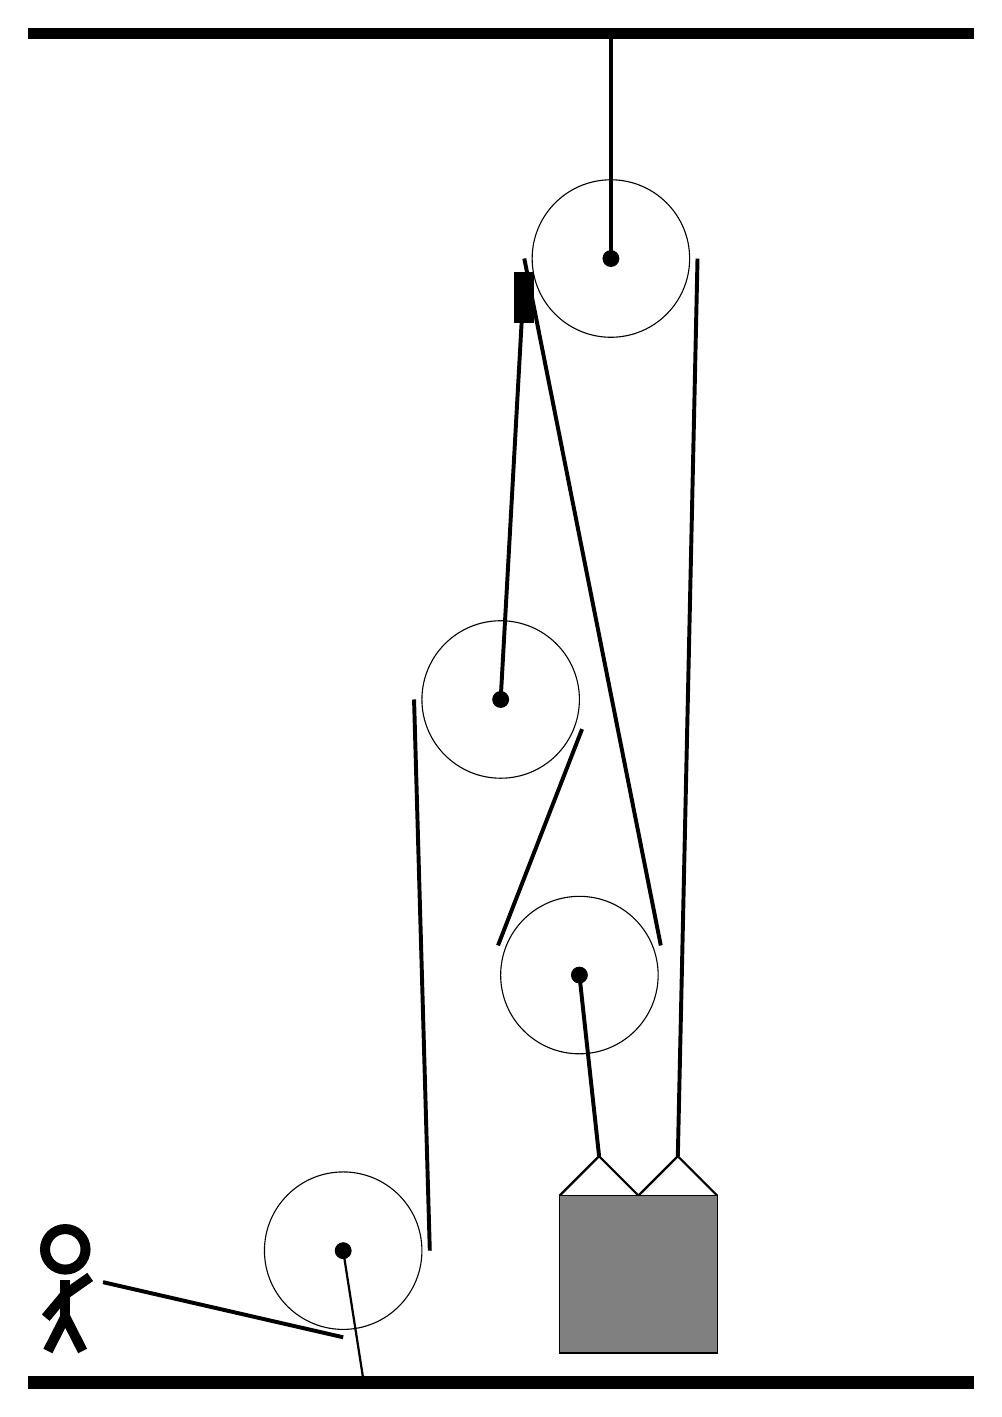
\begin{tikzpicture}
				\draw[fill=black] (-6, 14) rectangle (6, 14.125);
				
				\draw (0, 5.6) circle (1);
				\draw[fill=black] (0, 5.6) circle (0.1);
				
				\draw (1, 2.1) circle (1);
				\draw[fill=black] (1, 2.1) circle (0.1);
				
				\draw (1.4, 11.2) circle (1);
				\draw[fill=black] (1.4, 11.2) circle (0.1);
				\draw[very thick] (1.4, 11.2) -- (1.4, 14);
				
				\draw (-2, -1.4) circle (1);
				\draw[fill=black] (-2, -1.4) circle (0.1);
				\draw[thick] (-2, -1.4) -- (-1.75, -3);
				
				
				\draw[thick]  (0.75, -0.7) -- (1.25, -0.2) -- (1.75, -0.7) -- (2.25, -0.2) -- (2.75, -0.7);
				\draw[fill=black!50] (0.75, -0.7) rectangle (2.75, -2.7);
				\draw[line width=0.5mm] (-5.05, -1.8) -- (-2, -2.5);
				\centerarc[line width=0.5mm](-2, -1.4)(270:360:1.1);
				\draw[line width=0.5mm] (-0.9, -1.4) -- (-1.1, 5.6);
				\draw[line width=0.5mm] (0, 5.6) -- (0.3, 11.0);
				\draw[line width=0.5mm, fill=black](0.2, 10.4) rectangle (0.4, 11.0);
				\centerarc[line width=0.5mm](0, 5.6)(-20:180:1.1);
				\draw[line width=0.5mm] (1.0337, 5.2238) -- (-0.0337, 2.4762);
				\centerarc[line width=0.5mm](1, 2.1)(160:380:1.1);
				\draw[line width=0.5mm] (2.0337, 2.4762) -- (0.3, 11.2);
				\draw[line width=0.5mm](1, 2.1) -- (1.25, -0.2);
				\centerarc[line width=0.5mm](1.4, 11.2)(0:180:1.1);
				\draw[line width=0.5mm] (2.5, 11.2) -- (2.25, -0.2);
				
				\node at (-5.5, -1.9) {\scriptsize \Strichmaxerl[10][50][35]};
				
				\draw[fill=black] (-6, -3) rectangle (6, -3.15);
			\end{tikzpicture}
		\end{subfigure}
		\hfill
		\begin{subfigure}[b]{0.48\textwidth}
			\caption{Figure 2}
			\centering
			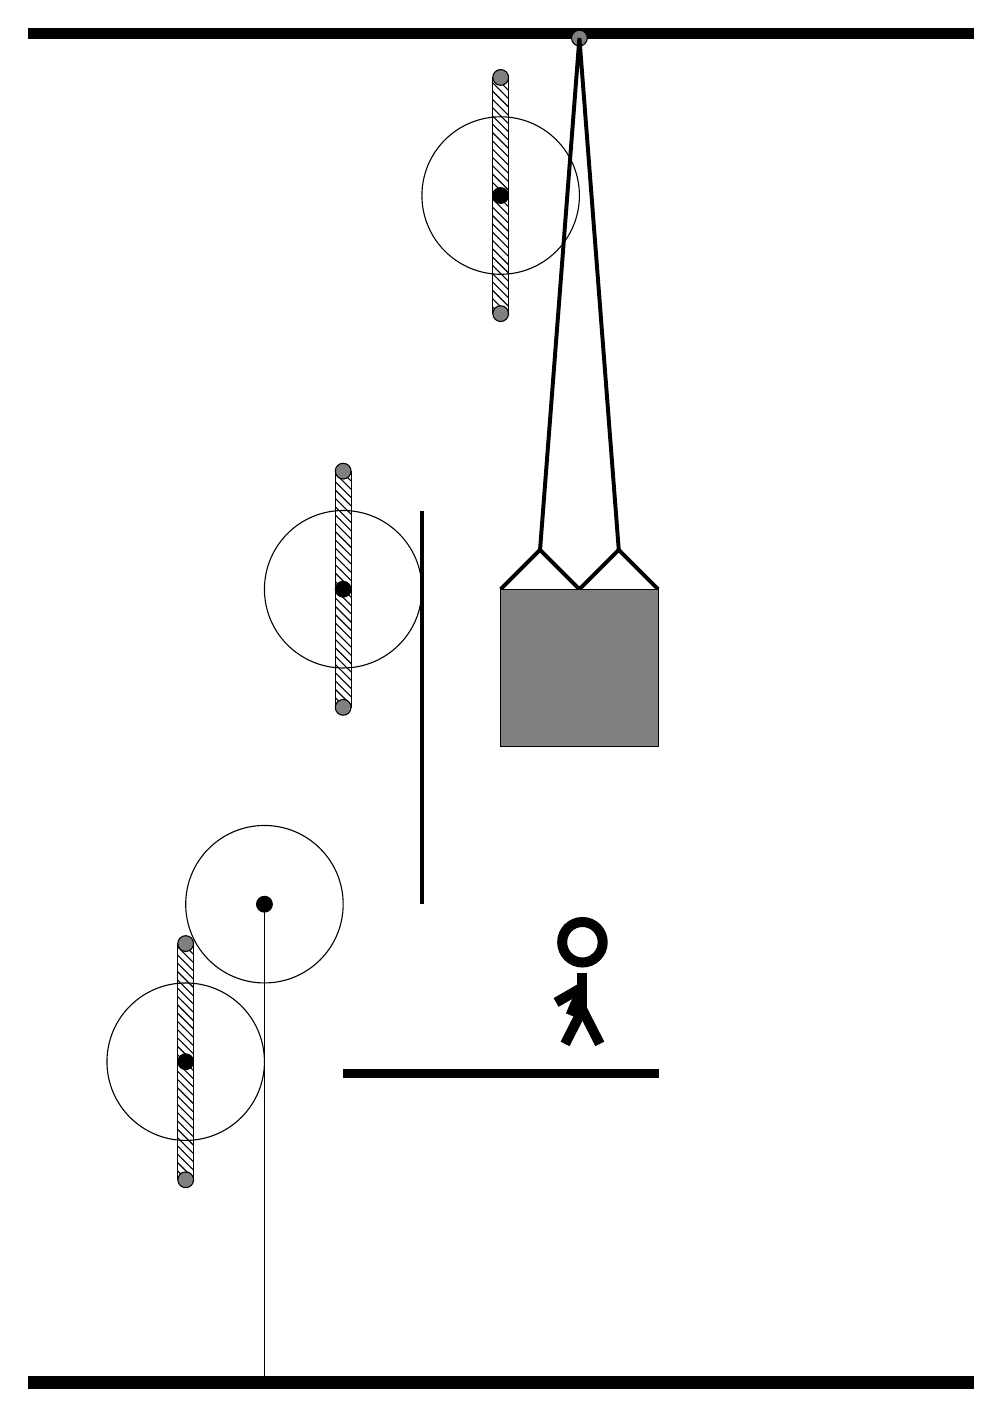
\begin{tikzpicture}
				\draw[fill=black] (-6, 14) rectangle (6, 14.125);
				
				\draw (-4,1) circle (1);
				\draw[fill=black] (-4,1) circle (0.1);
				\draw[pattern=north west lines, pattern color=black] (-4.1,2.5) rectangle (-3.9,-0.5);
				\draw[fill=black!50] (-4,2.5) circle (0.1);
				\draw[fill=black!50] (-4,-0.5) circle (0.1);
				
				\draw (0,12) circle (1);
				\draw[fill=black] (0,12) circle (0.1);
				\draw[pattern=north west lines, pattern color=black] (-0.1,13.5) rectangle (0.1,10.5);
				\draw[fill=black!50] (0,13.5) circle (0.1);
				\draw[fill=black!50] (0,10.5) circle (0.1);
				
				\draw (-2,7) circle (1);
				\draw[fill=black] (-2,7) circle (0.1);
				\draw[pattern=north west lines, pattern color=black] (-2.1,8.5) rectangle (-1.9,5.5);
				\draw[fill=black!50] (-2,8.5) circle (0.1);
				\draw[fill=black!50] (-2,5.5) circle (0.1);
				
				\draw (-3,3) circle (1);
				\draw[fill=black] (-3,3) circle (0.1);
				\draw (-3,-3.15) -- (-3,3);
				
				\draw[fill=black!50] (1,14) circle (0.1);
				\draw[line width=0.5mm](0.5,7.5) -- (1,14) --  (1.5,7.5);
				\draw[line width=0.5mm](0,7) --  (0.5,7.5) -- (1,7) -- (1.5,7.5) -- (2,7);
				\draw[fill=black!50] (0, 7) rectangle (2, 5);
				
				\draw[line width = 0.5mm] (-1,3) -- (-1,8);
				
				\node at (1, 2) {\scriptsize \Strichmaxerl[10][67][-150]};
				\draw[fill=black] (-2, 0.8999999999999999) rectangle (2, 0.8);
				
				\draw[fill=black] (-6, -3) rectangle (6, -3.15);
			\end{tikzpicture}
		\end{subfigure}
	\end{figure}
		\vspace*{\fill}
\end{document}